\chapter{\color{oxfordblue} Machine Learning \& Deep Learning}
\ChapFrame

\section{Introduction}
This chapter is entirely dedicated to a review of relevant \gls{ml} and \gls{dl} methods in the context of \gls{hep}. As for every other fields of science and technology, the recent advancements in the domain of \gls{ai} have introduced a shift of paradigm in particle physics. Before continuing with the review, some definitions of these different terms is suggested to decrypt their meaning.

\subsection{Definitions}
\subsubsection{Artificial Intelligence}
Artificial Intelligence encapsulates any piece of software, any \textit{programs}, that mimics an aspect of human intelligence. A non-exhaustive list of these aspects include: 
\begin{itemize}
    \item \textit{Reasoning}, the ability to conduct logical thoughts down to conclusions, 
    \item \textit{Inferring}, the ability to connect logical statements to induce new statements,
    \item \textit{Creativity}, the ability to generate new information. 
    \item \textit{Acting}, the ability to change the environment, particularly studied in the field of robotics. 
\end{itemize}
\gls{ai} is a large field of study that contains among many the area of robotics, natural language processing, computer vision, generative models, reinforcement learning. Artificial intelligence is broadly separated into three levels of performance, of which only the first one is currently accessible: 
\begin{enumerate}
    \item Narrow Intelligence: representing artificial intelligence capabilities on a specific problem, for which the underlying software is uniquely trained. This field includes \textit{reactive \gls{ai}}, where a model would be trained to output an optimal move based on current conditions only (e.g., the IBM chess player Deep Blue), and \textit{limited memory \gls{ai}}, where a model is able to draw knowledge from past data to make decision (e.g., any \gls{ml} model, such as the OpenAI chatGPT chat-box).
    \item Artificial General Intelligence: representing an artificial intelligence capable of matching human problem-solving skills. In particular, this hypothetical setting would let a machine learn new tasks on its own and extrapolate from its existing knowledge. 
    \item Artificial Super Intelligence: describes a hypothetical type of intelligence able to exceed human abilities and exhibit independent control of thoughts. 
\end{enumerate}

The inception of reactive \gls{ai} can be found in the research into games in the 50s and 60s. This approach saw the rise of algorithms capable of searching for the optimal move in large search spaces of possible actions using heuristics, human-passed knowledge of useful features of the specific environment of the game (e.g., the point system for chess pieces, with a queen being worth more than a simple pion). In this reactive approach, neither the rules of the game nor the decision process are learnt. The former is forced into the search logic and the latter is the outcome of the search process.

\subsubsection{Machine Learning} 
Machine Learning underpins the field of narrow \gls{ai} with limited memory capabilities. It represents a shift of paradigm in \gls{ai}: moving away from human-declared logic-based rules written in a specific syntax \[\textrm{\textit{If x happens, do y}},\] it automates the representation and update with mathematical models of both the dataspace ($\mathcal{D}$) and the learning process: \[\forall\, x \in \mathcal{D}, \textrm{ do }f(x) = \hat{y}; \textrm{ update }f(x) \textrm{ given } (x, y).\] In this respect, both the internal representation of the rules and the decision-making is underpinned by the trained mathematical model $f$.\\
Two general steps are combined into a model defined by learnable parameters: 
\begin{enumerate}
    \item Learning: the parameters of the model are updated based on a specified training or fit procedure, depending on whether the training will be progressively exposed to the data points of a training dataset or directly exposed to entirety of the set. The objective is to align the output of the model with the expected behaviour: given the couple $(x, y)$, let $f(x) = \hat{y} \rightarrow y$ under training convergence - this means the model $f$ has to become an unbias estimate of the label $y$. 
    \item Inferring: a trained model has to give its output on a new data point: $f(a) = \hat{b}$.
\end{enumerate}
The training process will depend on the type of model being deployed. These can be broadly separated into two fields:
\begin{itemize}
    \item Classical machine learning: includes decision trees (XGBoost, \gls{bdt} or \gls{mva}, random forest, ...), Support Vector Machine (SVM), logistic regression, kernel methods, ...
    \item Deep Learning (\gls{dl}): these methods are based on a core module call the Artificial Neural Network. This module is stacked into layers of given width, meaning a given number of neurons, and several layers of such modules are then connected along depth. 
\end{itemize}

\subsubsection{Deep Learning} 
Deep Learning corresponds to a specific set of methods who have quickly grown in popularity around 2010, with widely advertised results on competitive benchmark tasks in pattern recognition, as exemplified by the super-human performance of the \textit{DanNet} \cite{DanNet} model based on \gls{cnn}s \cite{NIPS198953c3bce6}. The basis of any \gls{dl} method is the Artificial Neural Network, a logical unit built to mimic the functioning of a human neuron. These neurons are then combined into layers of any numbers of neurons (the width of the layer) and the layers themselves are stacked into depth, with deeper layer receiving as input the output of earlier neurons. Different \gls{dl} models are constructed by modifying the structure of the layers - in particular, the input, output, and activation function used - and the transfer the information between neurons, be that between layers, depth-wise, or  between neurons, width-wise.\\
The task of a \gls{ml} model can be mutlifold the amount of human intervention \cite{MurphyML}: 
\begin{itemize}
    \item Classification: the task of assigning a label to a data sample, e.g., this jet is labelled a $b$-jet. The general case is multiclass, with $n$ labels possible, while a particular and common case is the binary classification case ($n = 2$).
    \item Regression: the task of predicting a continuous variable based on a data sample, e.g., the momentum of the particle is 15 GeV/$c$. 
    \item Feature extraction: given a dataset with specific features, reconstruct new features, e.g., given a set of tracks, reconstruct the secondary vertex. This case is a multidimensional case of regression combined with classificiation (do the tracks share a vertex?).
    \item Generation: given a sample of 1 million $t\bar{t}$ events, sample 10 new data points from the underlying statistical model. 
    \item Anomaly detection: identify and flag rare events in a dataset
\end{itemize}

There exist different paradigms of \gls{ml} models, divided mostly along the lines of the amount of human intervention \cite{MurphyML}:
\begin{itemize}
    \item \textit{Supervised learning}: the data used for training is endowed with the information the model must extrapolate. It is therefore restrain to generate information target directly by the learning process. Classificiation and regression are the most common examples.
    \item \textit{Unsupervised learning}: the data is not endowed with the information the model must learn to infer. The model is therefore trained with an objective to optimise without human intervention, and must discover patterns and insights without any guidance. Generative models and clsutering are prime examples.
    \item \textit{Semi-supervised learning}: also called \textit{weak supervision}, is a paradigm combining the two above. The model is mostly unsupervised but can benefit from some labelled cases or human input (a technique also named \textit{active learning}). A prime example is that a clustering tasks followed by a classification of the formed clusters. This is particularly fruitful when the cost of labelling the data is expensive, as is the case with real human data but thankfully not so in the case of particle physics data.
    \item\textit{Reinforcement Learning}: this paradigm of \gls{ml} is dedicated to the setting of a game theoretic environment. An agent must explore its environment and can act by choosing a specific policy. In \gls{rl}, the objective is for the agent to learn how to construct the most optimal policy to satisfy a reward function.
\end{itemize}

Given how important \gls{dl} methods have become in all technological fields, this chapter is primarily dedicated to introducing some of its approaches relevant to \gls{hep}. This form of \gls{ai} is indeed specifically well-suited to the setting of the \gls{atlas} experiment, as it enjoys:
\begin{itemize}
    \item large datasets of both real and simulated data are readily available,
    \item thanks to advanced \gls{mc}-based simulation programs, the simulated data points are faithful representations of the real data,
    \item the data and data-model from which the data originates is well understood in physics, the former coming from measurements from well-calibrated detectors and the second from crafted theories of the field. 
\end{itemize}


\section{Machine Learning Methods for Physics}
High-energy physicists enjoy a special relationship with \gls{ml} methods. Experimental particle physics largely relies on statistical analyses of complex and large datasets, be that simulated using \gls{mc} methods or collected from sophisticated detector apparata. A typical physics analysis can be described as the succession of four main steps:
\begin{enumerate}
    \item Data collection: real data is collected from a detector exposed to the underlying physics desired, e.g., at CERN placing and callibrating the \gls{atlas} detector at an interaction point of the \gls{lhc} to collect proton-proton collision data. 
    \item Simulated data is generated to match the condition of collection of the real data - in terms detector effects and operational conditions such as energy, \gls{pu} and luminosity. This simulated data englobes the best of our current theorical knowledge of the law of physics. 
    \item The detector of a modern particle physics experiment is a complex set of sub-detector system sensitive to different physical phenomena, as described in chapter %\ref{.}
    This low-level information collected by different device must be processed and recombine to generate \textit{objects}, aggregated information that often hold physical interpretation. For examples, from hits in the tracking detector a track can be fitted and some of its physical properties, such as \pt reconstructed. This task corresponding to a mapping from \textit{low}-level $\rightarrow$ \textit{high}-level measurement information can benefit from \gls{ml} in many ways. Broadly, \gls{ml}-based method can offer scalable, efficient, and precise solutions to this object reconstruction step. 
    \item An analysis strategy is established, with objective to similarly restrict the full dataset of both simulated and real data to a portion of the data-space that is most sensitive to the search signal or process. The sensitivity aspect underlies the need to take into account limited knowledge of the theorical physics, limited precision of the apparata, limited statistics of both simulations and data collected. To optimise the analysis, selection rules are derived based on physically accessible information, e.g., the centre-of-mass energy, presence of leptons, the transverse momentum \pt, and other high-level object reconstructed in the previous step.
    \item With the optimally selected set of real and simulated data, a statistical model is built to quantify the agreement of the measured data with the expectations from the theory under the conditions of the experiment. This is most often achieved through a likelihood computation.
\end{enumerate}

Modern advanced machine learning has the potential to improve all steps of this process:
\begin{enumerate}
    \item The operationial side of running the detector and the accelerator pipeline can benefit from \gls{rl} methods for improved control of the different electronic device. Triggers, an essential component of the \gls{atlas} experiment can be upgraded to use sophisticated \gls{dl} model running online thanks to a hardware back-bone built on \gls{fpga}s.
    \item Simulating a dataset through \gls{mc} approach is a computationally intensive task. Each event must pass through a selection of probabilistic step, with only a sastifying all requirements ending in the usable sample. This process can be speed-up and optimised significantly, but the costs remain significant to generate sample of sufficient statistics. Generative \gls{ai} has the potential to accelerate this step by giving statistical model that are possible to sample efficiently. \gls{gan} and \gls{vae} have been shown to perform the sampling step in a competitive amount of time. However, a key limitation of these stasticial approach is their limited ability to encorporate the sophisticated theorical model required to simulate the data, with any discrepancy or unclosure introducing levels of disagreement that are counter-productive for the final objective of the physics analyses.
    \item \gls{dl} is particularly well-suited for the object reconstruction task. Important examples in \gls{atlas} are identifying particles in the detector (e.g., $\tau$ identification), reconstructing missing transverse energe ($E_T$) in the triggers, and classifying heavy-flavour jets - as exemplified in the next chapter of this thesis dedicated to flavour tagging. 
    \item Historically, physicists have relied on a cut-base approach to select their data: they painfully analyse relevant variables to the physics problem to try and identify the best features to use to restrict the dataspace through manually-set restrictions. For example, in a measurement of $Z$-bosons decaying to two charged leptons $l^+l^-$ search, restricting the invariant mass of the lepton pair $m_{l^+l^-}$ to lie close the $Z$-boson rest mass $m_Z \approx 91.19$ GeV/$c^2$ is beneficial, as most of the search process will be found there. Machine learning is able to entirely bypass this need, learning directly from an appropriate set of signal and background datasets a transformation of the input data features to a discriminant optimising the separation of signal from background. 
    \item The likelihood function of the constructed statistical test, verifying the level of agreement between the real data and the theory through the simulated sample, can be directly learnt by a model given access to both sets. Furthermore, anamoly detection settings, such as those in the search for unknown resonances, can be derived using model \gls{ml} in an unsupervised setting, thereby automating the discovery process and requiring only real data. 
\end{enumerate}

One of the focus of this thesis can be broadly summarised as contributing to step 2 in the aformentioned list: developping \gls{dl}-tools for improved object reconstruction. The analysis presented in the latter part of this document also introduces some classical \gls{ml} technique of data selection - step 3. The rest of this chapter consists in a review of the relevant \gls{ml} methods. 

\subsection{Decision Trees}
\gls{dt}, also called textit{Classification and Regression Trees} (CART) are the bread and butter of any data analysis. They are simple to train, give a good ground performance for both classification and regression tasks, and are white box model - meaning they are easy to interpret. Underlying the model is a recursive partitioning approach of the input space \cite{MurphyML}. Labelling a partition step as \textit{node}, the tree structures emmerges from a \textit{root} state that is subsquently partitioned along different branches with one \textit{leaf} per final region. The splits are done along a feature of the input space, and the method accept both discrete categorical values (e.g., the label of a lepton as $e, \mu, \tau$) and continuous values (e.g., $m_l$). A simple classification tree structure can be represented as the following tree:

\Tree[.\textit{$x_i \leq c_i$} [.{True \\\textit{$x_j \geq c_j$}} [.True 1 ]
            [.False 0 ]]
        [.{False \\\textit{$x_k \leq c_k$}} [.True 0 ]
            [.{False \\{\textit{$x_l$} is \textit{$e$}}} [.True 0 ]
                            [.False 1 ]]]]

At each node there is a learnt condition with $x_i, x_j, x_k$ being continuous features of the dataset that are cut on $c_i, c_j, c_k$ and $c_l$ is a categorical feature (is the lepton an electron). The leaf values are the output of the tree in different regions defined by the combination of successive selections - here a binary variable. An example of a thus defined region is shown in Figure \ref{fig:tree-ex}, where a tree with two nodes is able to isolate most of the blue class from the red class with the region limited by green lines, corresponding to both conditions $x_1 \geq c_2$ and $x_2 \geq c_2$ being satisfied.

\begin{figure}[h!]
    \center
    \begin{minipage}[c]{0.3\textwidth}
        \caption{Binary classification with two features. A decision tree applies two successive cuts $c_1$ and $c_2$ to isolate the blue class from the red.}\label{fig:tree-ex}
      \end{minipage}
      \begin{minipage}[c]{0.5\textwidth}
        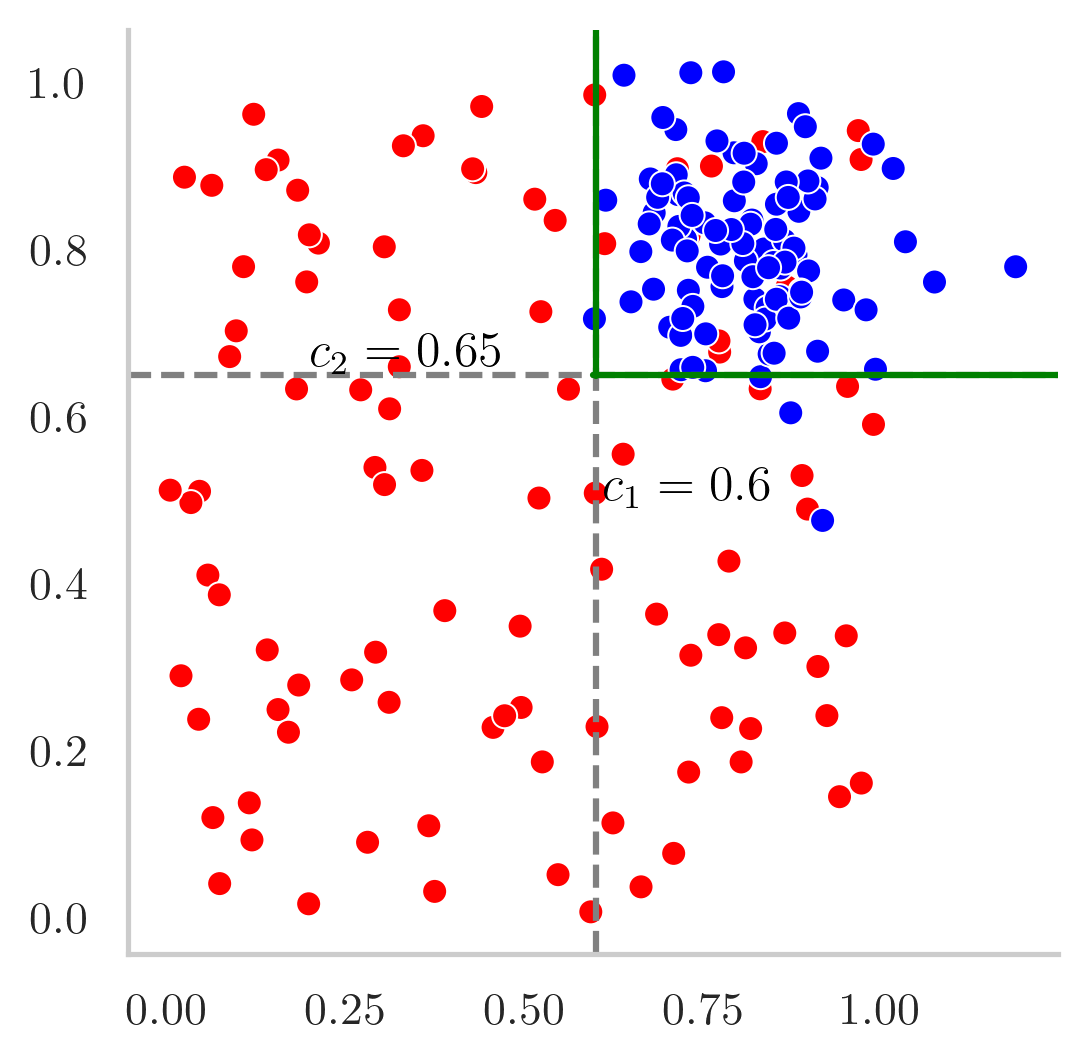
\includegraphics[width=\textwidth]{Images/ML/scatterPlot.png}
      \end{minipage}
\end{figure}

    
Finding the optimal set of partitions of a dataset is an NP-complete problem and therefore intractable for large datasets. To build a tree, a greedy approach must be adopted - meaning a heuristically successively choosing the most optimal step at each stage with no guarantee to find a local optimum with no guarantee of reaching a global optimum. The chosen split is selected based on a defined \textit{cost} by Equation \ref{eq:DTcost}.

\begin{equation}\label{eq:DTcost}
    (j^*, t^*) = \arg\min_{j\in \{1, ..., D\},\, t \in T_j} \min \left(\text{cost} (\{x_i, y_i : x_{ij} \leq t\}) + \text{cost}(\{x_i, y_i : x_j > t\}) \right)
\end{equation}
where $T_j$ is the set of possible thresholds, $x_j$, $y_j$ are the features and label (or regressive objective). For categorical variable, the inequality $x_j >< t$ would be typically converted in a value equality $x_j == t$. The \textit{cost} function will depend on the objective of the tree, with the regression case using the error function \[cost(D) : \sum_{i\in D}(y_i - \bar{y})^2,\] and for a classification the typical loss would be one of the following:
\begin{itemize}
    \item \textbf{Missclassification rate}: $\frac{1}{|D|} \sum_{i \in D} \mathbb{I}(y_i \neq \hat{y})$, where $D$ is the data in the leaf of the tree. 
    \item \textbf{Statistical entropy}: by defining the class-condidition probability $\pi_c = \frac{1}{|D|} \sum_{i \in D} \mathbb{I}((y_i) \neq c)$, where $\mathbb{I}$ is the identity function ($\mathbb{I}(x) = 1$ if $x$ is True, else $0$) the entropy over the ($C$) classes is defined as in Equation \ref{eq:statEntropy}. 
    \begin{equation}\label{eq:statEntropy}
        H(\vec{\pi}) = - \sum_{c=1}^C \pi_c \log \pi_c.
    \end{equation}
    \item \textbf{Information Gain}: an equivalent formulation to the entropy, where the gain in information that should be maximised is the relative change in entropy by adding a selection on feature $X_j$: 
    \[ \text{Gain}(X_j < t, Y) = H(Y) - H(Y | X_j < t) \]
    \item \textbf{Gini}: computes the expected error rate: \[\sum_{c=1}^C \pi_c (1 - \pi_c).\]
\end{itemize}


The pseudocode algorithm to train a \gls{dt} with this update rule is summarised in Algorithm \ref{ag:DT}. 

\begin{algorithm}
    \caption{Recursive Procedure to Train a Decision Tree \cite{MurphyML}}
    \begin{algorithmic}
    \Function{fitTree}{node, $D$, depth}
        \State $\text{node.prediction} \gets \text{mean}(\{y_i : i \in $D$\})$ 
        \State $(j^*, t^*, D_L, D_R) \gets \text{split}(D)$
        \If{\text{not worthSplitting}(\text{depth}, \text{cost}, $D_L$, $D_R$)}
            \State \Return node
        \Else
            \State node.left $\gets$ FITTREE(node, $D_L$, depth + 1)
            \State node.right $\gets$ FITTREE(node, $D_R$, depth + 1)
            \State \Return node
        \EndIf
    \EndFunction
    \end{algorithmic}
    \label{ag:DT}
\end{algorithm}

\gls{dt} can overfit a dataset and regularisation serves as an important step to avoid this unwanted behaviour. For trees, a natural procedure to avoid overtraining is to interrupt the growth of the tree when it is no longer worth doing so - a criterion that is hard to decide \textit{a priori} - or to \textit{prune} the tree, which implies the removes nodes or branches that contribute little to the overall performance. A simpler way to regularise the performance by reducing the variance of the estmate of the model is to train several trees with different subsets of the data chosen randomly with replacement and aggregate the results into a single prediction, for example by taking the average over each base learners: \[ y(x) = \frac{1}{N_l} \sum_{i=1}^{N_l} y_i(x),\] for $N_l$ base learner making prediction $y_i(x)$ given the input features $x$. This statistical technique of using ensemble of predictors is refered to as \textit{bagging}. To further decorrelate the performance of the different predictors, these can be reduced to a subset of the input features, thereby forming a \textit{random foret}.\\
For the following discussion, the model is built on a training dataset $ \{(x_1, y_1), ..., (x_N, y_N)\}$ with input vectors $x_i \in \{\mathbb{R} \otimes \mathbb{D}\}^d$ of $d$ features that are real or discrete ($\mathbb{D}$) and $y \in \mathbb{R}^d$ is a $d$-dimension real vector that serves as output to be predicted by the model.

\subsection{Boosted Decision Trees}
Another extension to the simple decision trees is to introduce the concept of \textit{boosting}, a method called Boosted Decision Trees (BDT) and, importantly in particle physics, \gls{mva}. Boosting is a greedy algorithm leveraging a weak learner or predictor (e.g., a \gls{dt}) and applying it sequentially to weighted versions of the data, with a larger weight given to missclassified / miss-regressed datapoints. This method is hugely popular in data science, having earned the title \textit{``best off-the-shelf classifier in the world''} \cite{baggingML}. Two particularly useful approaches are adaptive boosting (AdaBoost) \cite{Adaboost} and gradient boosting \cite{gradientBoosting}, both combining an ensemble of $L$ weak learners $f_i$ ($i = 1, ..., L$) into a strong learner \[F(x) = \sum_{i=1}^L f_i(x).\] 

\paragraph{AdaBoost:} combines the $L$ weak learners $h_i$ with adaptive weights $\alpha_i$ to improve the ensemble performance as \[\hat{f}(x) = \sum_{i=1}^L \alpha_i h_i(x),\] where $\hat{f}$ is the boosted model, and the successive boosting stages $f_T = \sum_{i=1}^{T \leq L} \alpha_i h_i(x)$ define stronger and stronger boosted variants of the model. At each iteration $m$ of the training process ($m = 1, ..., L$), a weight $w_i^m$ is assigned to each training sample (indexed by $i$) proportional to the current error or loss: $L(y_i, f_{t-1}(x_i))$, where the typical case for AdaBoost is binary classification with $y_i \in {-1, 1}$. The error in AdaBoost is the exponential loss on the datapoint of Equation \ref{eq:adaboosterror}. 

\begin{equation}\label{eq:adaboosterror}
    E = L(y, f_m(x)) = \sum_{i=1}^N \exp\left(-y_i f_m(x_i)\right) = \sum_{i=1}^N \exp\left(-y_i (f_{m-1}(x_i) + \alpha_m h_m(x_i))\right)
\end{equation}
Equation \ref{eq:adaboosterror} can be re-expressed to highlight the weight $w_{i,m}$ applied to each datapoint $(x_i, y_i)$ at step $m$ as : \[\sum_{i=1}^N w_{i,m} \exp\left(-\alpha_m y_i h_m(x_i)\right),\] where $w_{i,m} = \exp\left(-y_i f_{m-1}(x_i)\right)$. \\
The weak learner at step $m$ is applied to the weighted version of the dataset with weights $w_{i,m}$ with optimal weights $\alpha_m$ found by minimising the error to be \[\alpha_m = \frac{1}{2} \log \frac{1 - \epsilon_m}{\epsilon_m},\] where $\epsilon_m$ is the ratio of miss-classified weights: $\epsilon_m = \sum_i w_{i,m} \mathbb{I}(y_i \neq h_m(x_i)) / \sum_i w_{i,m}$. The AdaBoost algorithm is summarised in Algorithm \ref{algo:adaboost}.

\begin{algorithm}
    \caption{Adaboost for Binary Classification with Exponential Loss \cite{MurphyML}}
    \label{algo:adaboost}
    \begin{algorithmic}
    \State Initialize weights: $w_i = \frac{1}{N}$, where $N$ is the number of samples.
    \For{$m = 1$ to $M$}
        \State Fit a classifier $h_m(x)$ to the training set using weights $w$.
        \State Compute $\epsilon_m = \sum_i w_{i,m} \mathbb{I}(y_i \neq h_m(x_i)) / \sum_i w_{i,m}$.
        \State Compute $\alpha_m = \log\left(\frac{1 - \epsilon_m}{\epsilon_m}\right)$.
        \State Update weights: $w_i \leftarrow w_i \, \exp(\alpha_m \cdot \mathbb{I}(y_i \neq h_m(x_i)))$.
    \EndFor
    \State \Return $f(x) = \text{sgn}\left(\sum_{m=1}^M \alpha_m h_m(x)\right)$
    \end{algorithmic}
\end{algorithm}

\paragraph{Gradient boosting:} is a generic approach which does not require a specific derivation for each loss function. The objective is to minimise the empirical risk, the expected value of the loss function $L$ on the training set as shown in Equation \ref{eq:empRisk}: 
\begin{equation}\label{eq:empRisk}
    \hat{f}  = \arg \min_f \mathbb{E}_{x,y} L(y, f(x))
\end{equation}
where $f(x) = (f(x_1), ..., f(x_N))$ is the output of the learner on the training set. As the name suggests, the approach leverages gradient descent to find the optimal $\hat{f}$. At step $m$, the gradient of the loss $L(f)$ is evaluated at $f = f_{m-1}$ as \[ g_{i,m} = \left[ \frac{\partial  L(y_i, f(x_i))}{\partial f(x_i)} \right]_{f= f_{m-1}}, \] which is then used to update the learner with a step \[ f_m = f_{m-1} - \alpha g_{m}\] of step-length $\alpha_m$ chosen to minimise the residual loss $L(y, f_{m-1} - \alpha_m g_{m})$. 

For the specific case of gradient boosted decision trees, at step $m$ a \gls{dt} $h_m(x)$ is fitted to the pseudo-residuals. This \gls{dt} $h_m$ at step $m$ defines $J_m$ disjoint regions through its leaves with predictions $b_{jm}$ in each $j = 1, ... J_m$ regions: \[ h_m(x) = \sum_{j=1}^{J_m} b_{jm} \textbf{1}_{R_{jm}}(x),\] where $\textbf{1}_{R_{jm}}(x)$ is the indicator function - equals to 1 when $x \in R_{jm}$ and 0 otherwise. The update to the model is chosen so that: \[f_m(x) = f_{m-1} + \gamma_m h_m(x),\] with $\gamma_m$ selected by minimising the empirical risk of the updated model: \[ \gamma_m = \arg \min_{\gamma} \sum_{i=1}^N L(y_i, f_{m-1}(x_i) + \gamma h_m(x_i)).\]

\begin{algorithm}
    \caption{Gradient Boosting \cite{MurphyML}}
    \label{algo:gradient_boosting}
    \begin{algorithmic}
    \State Initialize $f_0(x) = \arg\min_\alpha \,\sum_{i=1}^N L(y_i, h(x_i; \alpha))$
    \For{$m = 1$ to $M$}
        \State Compute the gradient residual $\forall i$: $g_{i,m} = -\left[\frac{\partial L(y_i, f(x_i))}{\partial f(x_i)}\right]_{f(x_i) = f_{m-1}(x_i)}$
        \State Train weak learner $h_m$ on the dataset $\{(x_i, r_{i,m})\}_{i=1}^N$
        \State Compute $\alpha_m$ by minimising $\sum_{i=1}^N(g_{i,m} - \alpha_m h_m(x_i))$
        \State Update $f_m(x) = f_{m-1}(x) + \nu \alpha_m h_m(x)$
    \EndFor
    \State \Return $f(x) = f_M(x)$
    \end{algorithmic}
\end{algorithm}

The full algorithm for Gradient Boosting is mentioned in Algorithm \ref{algo:gradient_boosting}, where the update rule is added a \textit{learning rate} hyperparameter $\nu$ to introduce regularisation and reduce the risk of overfitting. By keeping $0 < \nu \leq 1$, reduces the ability of the model to fully adapt to the training error, thereby improving generalisation. The price is a slower updating of the model and therefore a more demanding computational time. Further regularising techniques are bootstrap aggregation - training each weak learn on a random subset of the data -, limiting the number of leaves, or more generally penalising model of larger complexity - removing branches that do not reduce the loss by a minimal amount. 

\gls{bdt} resist better to overtraining thanks to the regularisation effect of boosting and the different techniques described in thi section. An undiserable feature of boosting is the loss of direct interpretability of the decision. 

\subsection{Artificial Neural Network}

\subsection{Multilayer Perceptron}

\subsection{Recurrent Neural Network}

\subsection{Convolutional Neural Network}

\subsection{Graph Neural Network}

\subsection{The rise of the Transformer}

\subsection{Generative Models: GAN \& VAE}

\subsection{Reinforcment Learning}

\section{Training and Optimising Deep Learning Models}

